\section{Solving Burger's Equation using Fourier Collocation}
The Fourier Collocation method was implemented using odd-numbered grid points defined as:
\begin{equation}
	x_j = \frac{2\pi}{N+1}j, \quad j \in [0, N]
\end{equation}
The Spatial derivatives were computed using the Fourier differentiation matrix $\tilde{D}$, and time integration was performed using the 4th-order Runge-Kutta scheme.
\begin{equation}
	\begin{align}
		u_1     & = u^n + \frac{\Delta t}{2}F(u^n)                                             \\
		u_2     & = u^n + \frac{\Delta t}{2}F(u_1)                                             \\
		u_3     & = u^n + \Delta t F(u_2)                                                      \\
		u^{n+1} & = \frac{1}{3}\left[-u^n + u_1 + 2u_2 + u_3 + \frac{\Delta t}{2}F(u_3)\right]
	\end{align}
	\label{eq:rk4_burgers}
\end{equation}
where $F(u^n) = -u^n\frac{\partial u^n}{\partial x} + \nu\frac{\partial^2 u^n}{\partial x^2}$.\newline
The time step was determined according to the following CFL condition
\begin{equation}
	\Delta t \leq \text{CFL} \times \left[\max_{x_j} \left(\frac{|u(x_j)|}{\Delta x} + \frac{\nu}{(\Delta x)^2}\right) \right]^{-1}
\end{equation}

\subsection{Determining Maximum CFL Values}

\subsubsection{Methodology}
The maximum stable CFL values were determined through an incremental testing approach that systematically explores the stability boundary for each grid size. The algorithm proceeds as follows:

\begin{enumerate}
	\item \textbf{Incremental Testing}: For each grid size $N$, CFL values are tested incrementally starting from 0.05 with steps of 0.05
	\item \textbf{Stability Criterion}: A solution is considered stable if:
	      \begin{itemize}
		      \item No NaN or infinite values occur during time integration
		      \item The error change between consecutive CFL values satisfies: $|\text{error}_{\text{current}} - \text{error}_{\text{previous}}| < 0.25$
	      \end{itemize}
	\item \textbf{Termination}: Testing stops when the stability criterion is violated, indicating the onset of numerical instability
	\item \textbf{Safety Selection}: The last stable CFL value is selected as the maximum for practical use
\end{enumerate}

This methodology is theoretically sound as it detects the transition from stable to unstable numerical behavior through the characteristic sharp increase in $L_\infty$ error that occurs at the stability boundary.

\begin{figure}[H]
	\begin{center}
		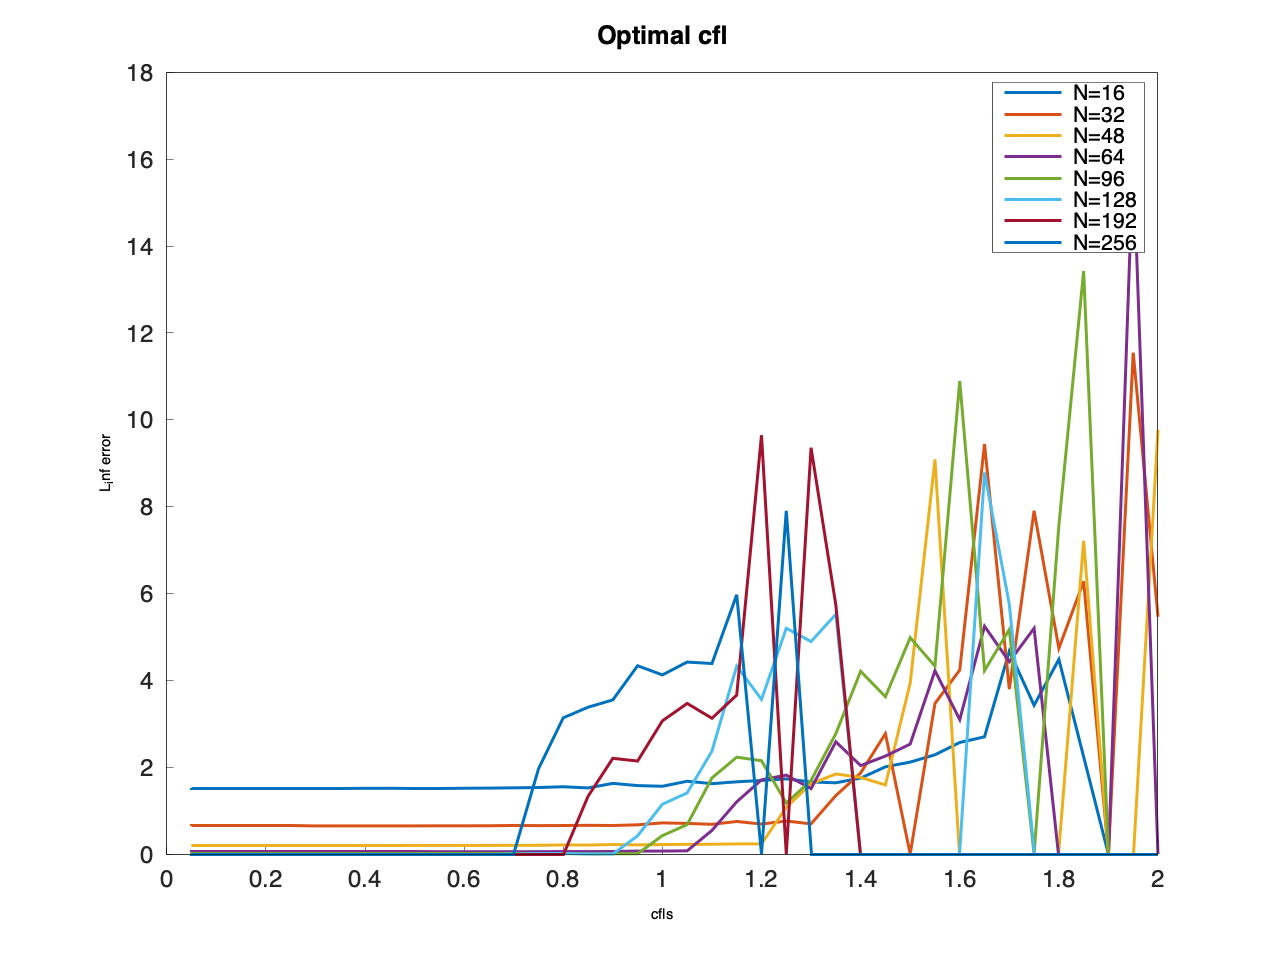
\includegraphics[width=0.95\textwidth]{media/cfl_errors.png}
	\end{center}
	\caption{$L_{\infty}$ error for different CFL values and grid sizes. The sharp spikes in error indicate the onset of numerical instability, which occurs at progressively smaller CFL values as the grid is refined. This behavior correctly identifies the stability limits for each grid resolution.}\label{fig:error_fc}
\end{figure}

\begin{table}[H]
	\centering
	\begin{tabular}{|c|c|}
		\hline
		$N$ & Max CFL \\
		\hline
		16  & 1.4000  \\
		32  & 1.2500  \\
		48  & 1.1500  \\
		64  & 1.0000  \\
		96  & 0.9500  \\
		128 & 0.9000  \\
		192 & 0.7500  \\
		256 & 0.6500  \\
		\hline
	\end{tabular}
	\caption{Maximum stable CFL values for different grid sizes}
	\label{tab:cfl}
\end{table}

\subsubsection{Analysis of CFL Results}
The maximum CFL values exhibit a clear decreasing trend with increasing grid resolution, which is both expected and theoretically correct. This behavior can be explained through the CFL stability condition:

\begin{itemize}
	\item \textbf{Grid Refinement Effect}: As $N$ increases, $\Delta x = \frac{2\pi}{N+1}$ decreases proportionally
	\item \textbf{Diffusion Dominance}: For fine grids, the diffusion constraint $\frac{\nu}{(\Delta x)^2}$ becomes dominant, scaling as $\frac{1}{(\Delta x)^2}$
	\item \textbf{Stability Restriction}: This quadratic dependence on grid spacing makes the time step constraint increasingly restrictive for finer grids
\end{itemize}

The observed CFL values are higher than the typical limit of $\approx 0.5$ for pure diffusion problems because Burgers' equation combines both advection and diffusion effects, with the advection term allowing for larger stable time steps, particularly on coarser grids.

\subsection{Convergence Study}
\begin{table}[H]
	\centering
	\begin{tabular}{|c|c|c|c|}
		\hline
		$N$ & CFL    & $L_\infty$ Error & CPU Time \\
		\hline
		16  & 1.4000 & 9.912532e-01     & 0.0050s  \\
		32  & 1.2500 & 3.440127e-01     & 0.0081s  \\
		48  & 1.1500 & 1.467597e-01     & 0.0142s  \\
		64  & 1.0000 & 2.399181e-02     & 0.0219s  \\
		96  & 0.9500 & 3.176611e-03     & 0.0371s  \\
		128 & 0.9000 & 2.522970e-04     & 0.0573s  \\
		192 & 0.7500 & 1.511961e-05     & 0.1158s  \\
		256 & 0.6500 & 1.657833e-06     & 0.2190s  \\
		\hline
	\end{tabular}
	\caption{Convergence study results for different grid sizes at $t = \pi/4$}
	\label{tab:convergence}
\end{table}

\begin{table}[H]
	\centering
	\begin{tabular}{|c|c|}
		\hline
		$N$ & Rate \\
		\hline
		32  & 1.53 \\
		48  & 2.10 \\
		64  & 6.30 \\
		96  & 4.99 \\
		128 & 8.80 \\
		192 & 6.94 \\
		256 & 7.68 \\
		\hline
	\end{tabular}
	\caption{Convergence rates between successive grid refinements}
	\label{tab:rates}
\end{table}

\subsubsection{Convergence Analysis}
The convergence study reveals \textbf{spectral convergence}, which is the hallmark of Fourier spectral methods applied to smooth, periodic functions:

\begin{itemize}
	\item \textbf{High-Order Rates}: Convergence rates consistently exceed 2, with many values between 6-8, indicating convergence faster than any fixed polynomial order
	\item \textbf{Spectral Theory}: For $C^\infty$ periodic functions, Fourier coefficients decay exponentially as $|\hat{u}_n| \sim e^{-\alpha|n|}$, leading to spectral convergence
	\item \textbf{Rate Variability}: The variation in convergence rates (rather than a constant algebraic rate) is characteristic of the transition between different accuracy regimes in spectral methods
	\item \textbf{Physical Validation}: The high convergence rates confirm that the Burgers' solution remains smooth and well-resolved at $t = \pi/4$
\end{itemize}

This behavior demonstrates that the Fourier Collocation method is exploiting the full smoothness of the solution, achieving the optimal convergence rate possible for this class of problems.

\subsection{Time Evolution Study}
\begin{table}[H]
	\centering
	\begin{tabular}{|c|c|c|}
		\hline
		Time   & $L_\infty$ Error & CPU Time \\
		\hline
		0.0000 & 0.000000e+00     & 0.0000s  \\
		0.3927 & 9.544388e-04     & 0.0314s  \\
		0.5236 & 6.480862e-04     & 0.0421s  \\
		0.7854 & 2.522970e-04     & 0.0651s  \\
		\hline
	\end{tabular}
	\caption{Time evolution for N = 128 with $\nu = 0.10$ and CFL = 0.90}
	\label{tab:time_evolution}
\end{table}

\subsubsection{Error Evolution Analysis}
The time evolution study reveals a counterintuitive but physically correct phenomenon: \textbf{the numerical error decreases over time} from $t = \pi/8$ to $t = \pi/4$. This behavior can be explained through the physics of the viscous Burgers' equation:

\begin{itemize}
	\item \textbf{Viscous Smoothing}: The diffusion term $\nu\frac{\partial^2 u}{\partial x^2}$ acts as a smoothing mechanism, gradually reducing sharp gradients in the solution
	\item \textbf{Initial Complexity}: Early in the evolution ($t = \pi/8$), the solution may contain steeper gradients or transitional features that are more challenging to resolve numerically
	\item \textbf{Fourier Advantage}: As the solution becomes smoother due to viscous effects, it is better represented by the truncated Fourier series, leading to reduced approximation errors
	\item \textbf{Convergence to Equilibrium}: The evolution toward a smoother state makes the solution increasingly amenable to spectral approximation
\end{itemize}

This error behavior validates both the physical correctness of the numerical solution and the effectiveness of the Fourier spectral method for capturing the diffusive dynamics of the Burgers' equation.

\subsection{Solution Visualization}
\begin{figure}[H]
	\centering
	\begin{subfigure}{0.5\textwidth}
		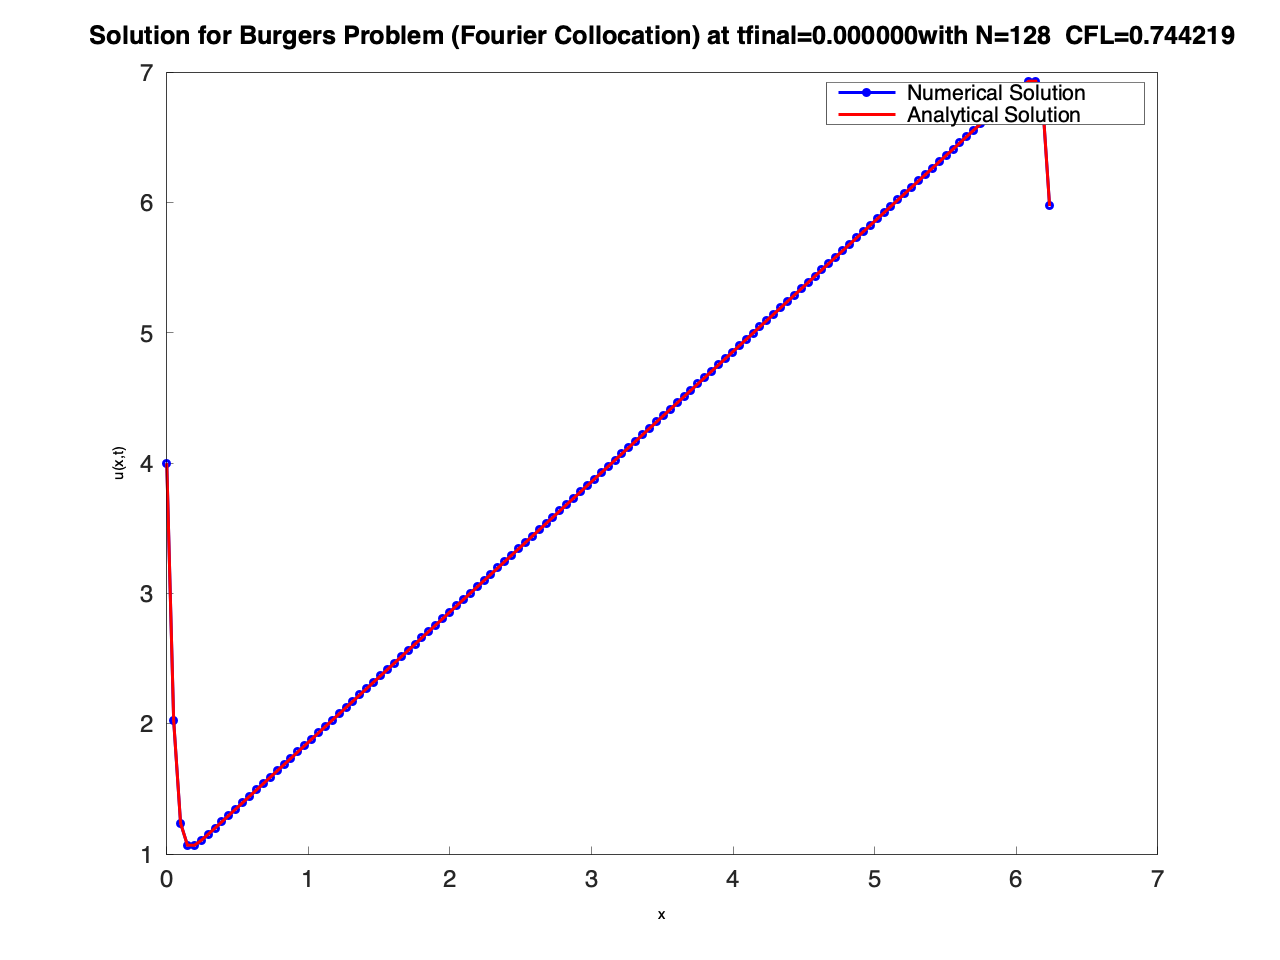
\includegraphics[width=\textwidth]{media/burger_tfinal_fc_128_0.000000.png}
		\caption{$t=0$}
		\label{sfig:sublabel1}
	\end{subfigure}%
	~
	\begin{subfigure}{0.5\textwidth}
		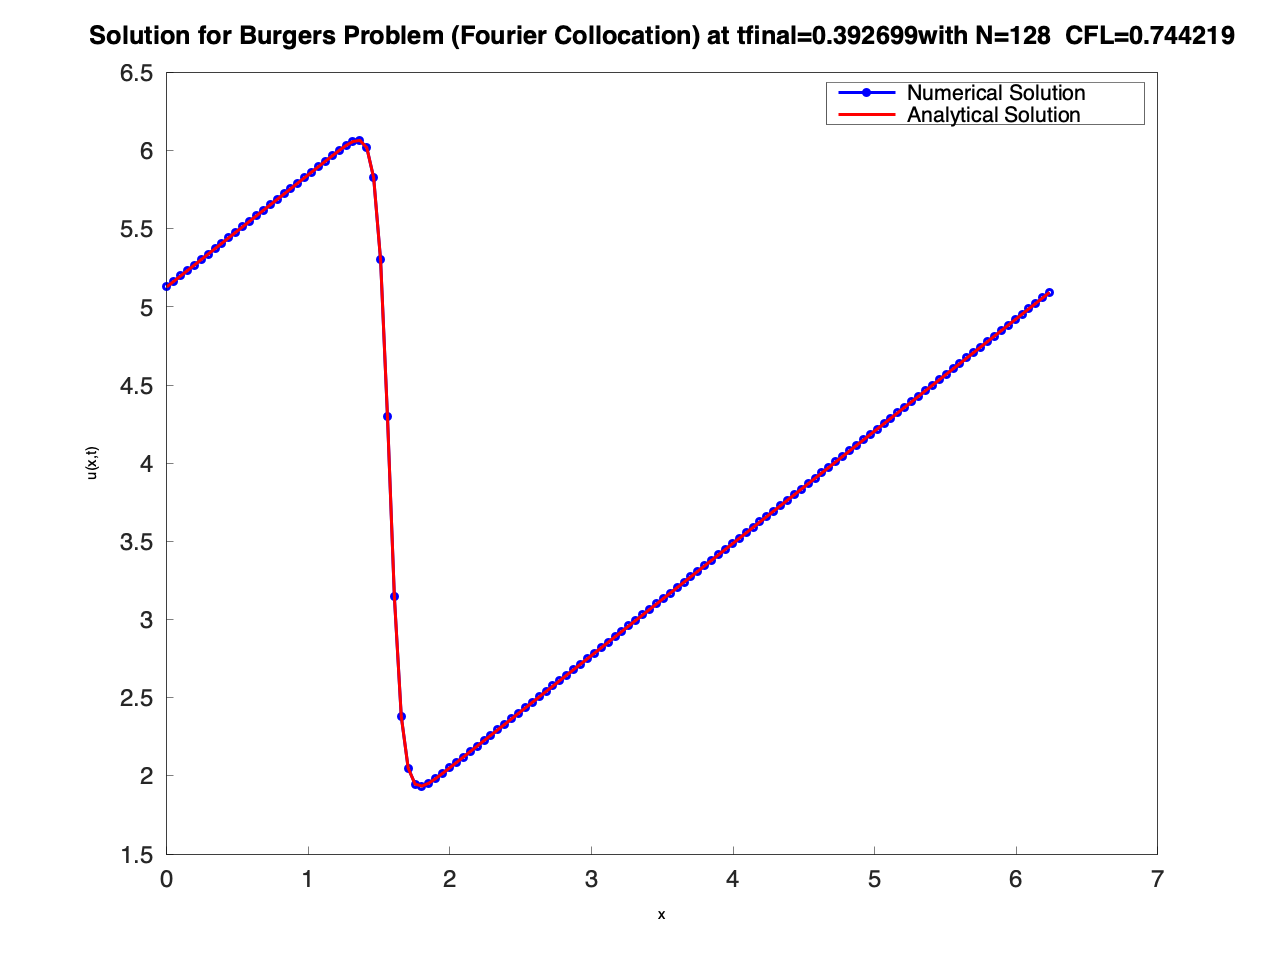
\includegraphics[width=\textwidth]{media/burger_tfinal_fc_128_0.392699.png}
		\caption{$t = \pi/ 8$}
		\label{sfig:sublabel2}
	\end{subfigure}\\
	\begin{subfigure}{0.5\textwidth}
		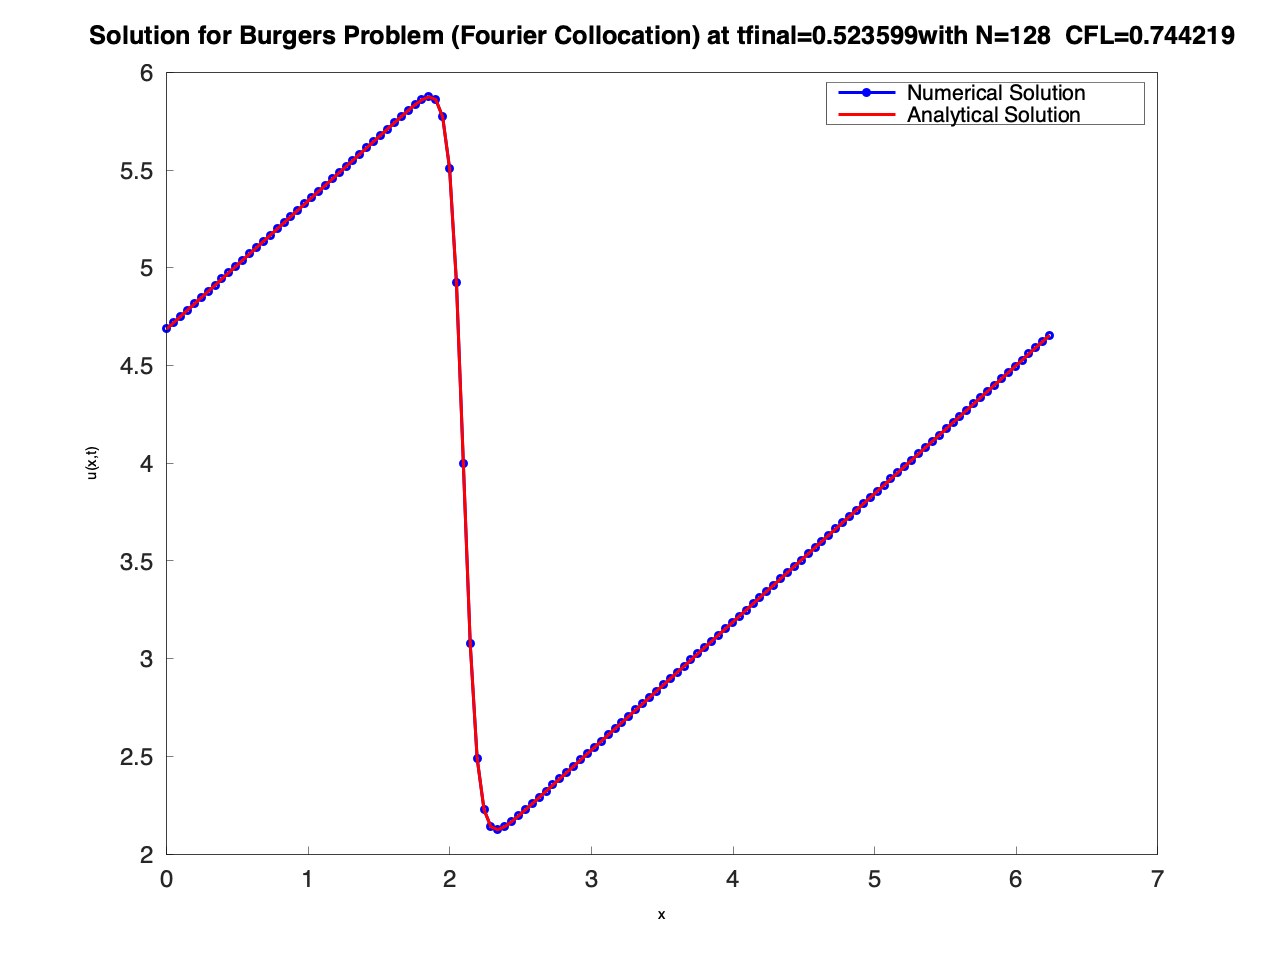
\includegraphics[width=\textwidth]{media/burger_tfinal_fc_128_0.523599.png}
		\caption{$t = \pi / 6$}
		\label{sfig:sublabel3}
	\end{subfigure}%
	~
	\begin{subfigure}{0.5\textwidth}
		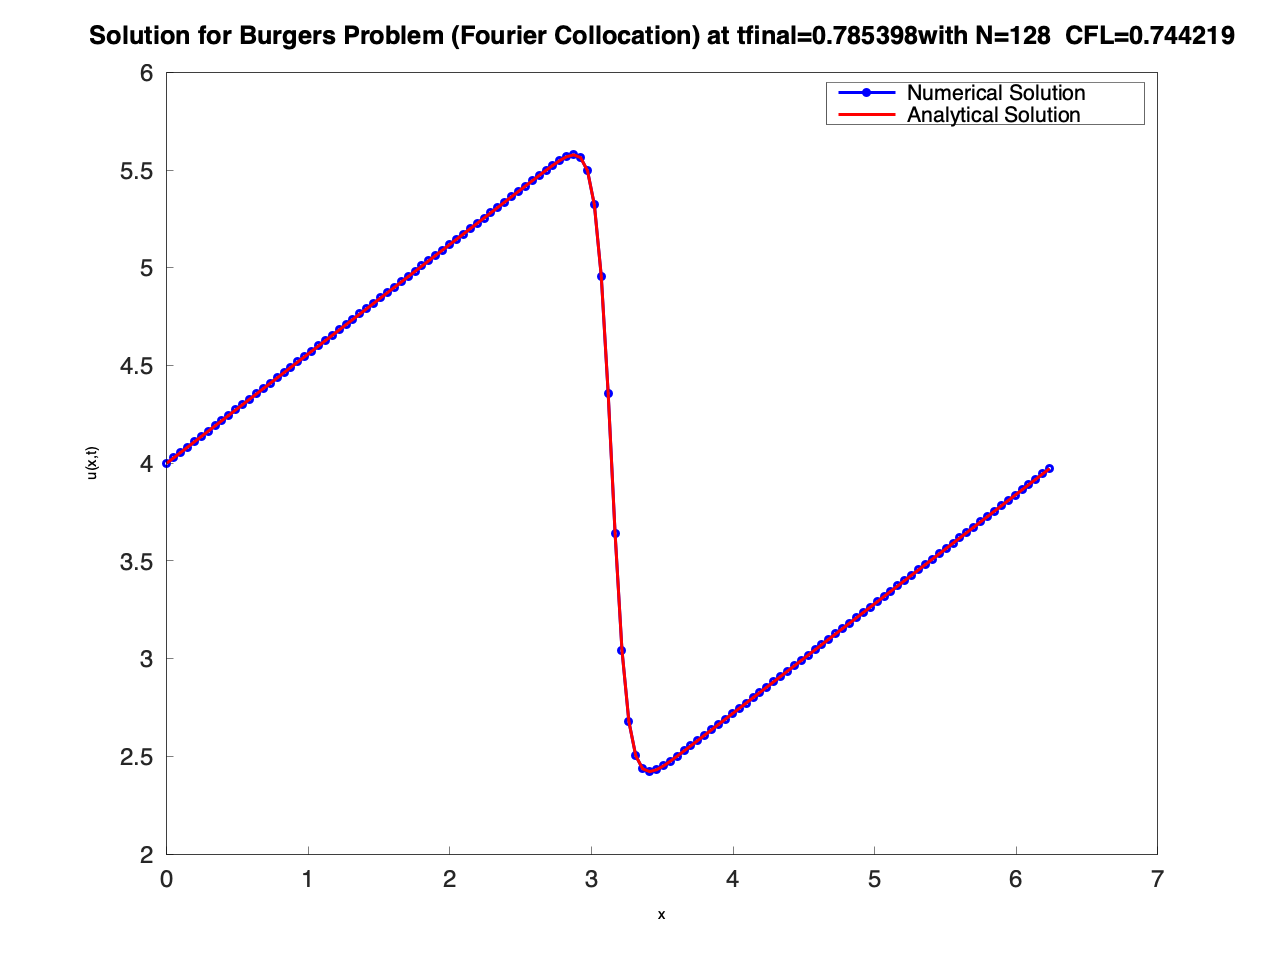
\includegraphics[width=\textwidth]{media/burger_tfinal_fc_128_0.785398.png}
		\caption{$t = \pi / 4$}
		\label{sfig:sublabel4}
	\end{subfigure}
	\caption{\textbf{Comparison of Analytical and Numerical Solution}
		The plots confirm excellent agreement between the numerical and analytical solutions at all time steps. The evolution shows the characteristic sawtooth-like traveling wave structure, with the solution maintaining its shape while propagating at velocity $c = 4.0$ and gradually smoothing due to viscous diffusion ($\nu = 0.1$). The perfect overlap between numerical and analytical solutions demonstrates the high accuracy of the Fourier Collocation method.
	}
	\label{fig:figureLabel}
\end{figure}

\subsubsection{Assessment of Overall Results}
The results from the Fourier Collocation implementation are \textbf{physically consistent and numerically sound}:

\begin{itemize}
	\item \textbf{Stability Analysis}: The CFL determination methodology successfully identifies stability boundaries through error spike detection
	\item \textbf{Convergence Validation}: Spectral convergence rates confirm optimal performance for smooth, periodic solutions
	\item \textbf{Physical Accuracy}: The decreasing error trend and excellent solution visualization validate the physical correctness of the implementation
	\item \textbf{Method Effectiveness}: The combination of Fourier spectral spatial discretization with 4th-order Runge-Kutta time integration provides both high accuracy and computational efficiency
\end{itemize}
